\section{Altitude keeping}
\begin{marginfigure}
	\centering
	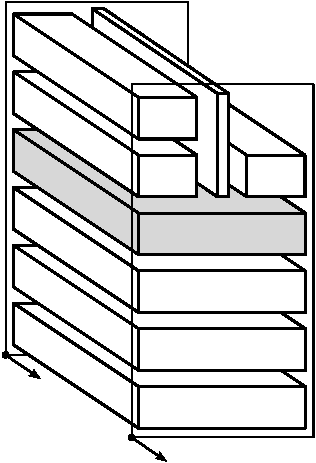
\includegraphics[scale=0.5]{ch3/img/PA_map_altitude.pdf}
\end{marginfigure}
The last basic block that should be implemented is the altitude keeping, to maintain the distance of the drone to the soil high enough to avoid contact with rescuer and low enough to get a good signal strength. The sensors used are, again, ultrasonic range finder. With respect to the obstacle avoidance, that acts as a control on the lateral dynamic of the drone, that is quite slow, altitude keeping works on vertical dynamic that is really fast, and need a more reliable implementation, and require a statistical system to determine the distance even with a high irregular terrain.

This part was actually not implemented because of the need of more test about response of ultrasonic waves upon snow surface, to better understand the effects of density on perceived distance.

\subsection{Kalman Filter}
We assume that the dimension could be described with the use of normal distribution:
\begin{equation}
p(\hexastate) \det\braces{(2\pi)^{n}\Sigma_0}^{-1/2} e^{-\dfrac{1}{2}\braces{\hexastate - \boldsymbol{\mu}}^T \Sigma^{-1}\braces{\hexastate - \boldsymbol{\mu}}}
\end{equation}
with ${\boldsymbol{\mu}}$ the mean value for the distribution and ${\Sigma}$ covariance matrix of the distribution.

The Kalman filter include the knowledge of the covariance matrix into the state estimation procedure, and it is possible to proof that the final estimation will maintain a normal distribution if:
\begin{itemize}
\item distribution of initial state is normal
\item the state distribution is a linear function of the previous state and a white Gaussian noise
\item the measurement distribution  is a linear function of the state and a white Gaussian noise
\end{itemize}

\myparagraph{Initial state probability}
We make the really strong hypothesis to have an initial distribution in the normal form:
\begin{equation}
p(\hexastate_0) \det\braces{(2\pi)^{n}\Sigma_0}^{-1/2} e^{-\dfrac{1}{2}\braces{\hexastate_0 - \boldsymbol{\mu_0}}^T \Sigma_{0}^{-1}\braces{\hexastate_0 - \boldsymbol{\mu_0}}}
\end{equation}

\myparagraph{Prediction phase}
The distribution of the state derives from the distribution of the previous state, using the linear relation:
\begin{equation}
\hexastate_t = A_t \hexastate_{t-1} + B \hexacontrol_t + \statenoise
\end{equation}
where ${\mathbf{w}_t}$ is a realization of a distribution ${\mathcal{N}(\mathbf{0},R_t)}$ in which $R_t$ is the matrix that describes the covariance of the noise on the state.

The distribution is normal due to the relations:
\arraymath{
\bar{\boldsymbol{\mu}_{t}} &=& A_t \boldsymbol{\mu}_{t-1} + B_t \hexacontrol_{t} \\
\bar{\Sigma_{t}} &=& A_t \Sigma_{t-1} A_t^T + R_t \\
p(\hexastate_t \mid \hexastate_{t-1}, \hexacontrol_t) &=& \det((2\pi)^n R_t)^{-\frac{1}{2}} e^{\left( - \frac{1}{2} (\hexastate_t - \bar{\boldsymbol{\mu}_{t}})^T {R_t}^{-1} (\hexastate_t - \bar{\boldsymbol{\mu}_{t}}) \right)}
}

If the system has a non--linear function that describes the dynamic, it could be approximated with a first--order Taylor expansion:
\begin{equation}
\hexastate_t = g\braces{\hexastate_{t-1},\hexacontrol_t} + \statenoise
\end{equation}
\arraymath{
\mathrm{Taylor}_{1}\left(g(\hexastate_{t-1},\hexacontrol_t)\right)\Big\rfloor_{\bar{\boldsymbol{\mu}}_{t-1},\bar{\hexacontrol}_t} & = & g(\bar{\boldsymbol{\mu}}_{t-1},\bar{\hexacontrol}_t) + \\ & & \nabla_{\hexastate} g (\hexastate_{t-1},\hexacontrol_t)\Big\rfloor_{\bar{\boldsymbol{\mu}}_{t-1},\bar{\hexacontrol}_t}\left( {\hexastate}_{t-1} - \bar{\boldsymbol{\mu}}_{t-1} \right) \\
& = & g(\bar{\boldsymbol{\mu}}_{t-1},\bar{\hexacontrol}_t) + A_t\left( {\hexastate}_{t-1} - \bar{\boldsymbol{\mu}}_{t-1} \right)
}

\myparagraph{Estimation state}
The measurement distribution derives directly from the measurement model:
\begin{equation}
\mathbf{z}_t = C_t \hexastate_t + \measnoise
\end{equation}
where ${\mathbf{v}_t}$ is a realization of a distribution ${\mathcal{N}(\mathbf{0},Q_t)}$ in which $Q_t$ is the matrix that describes the covariance of the noise on the measurement.

The distribution maintains its normal behavior due to the relation:
\[p(\mathbf{z}_t\mid\hexastate_t) = \det((2\pi)^n Q_t)^{-\frac{1}{2}} e^{\left( -\frac{1}{2} (\mathbf{z}_t - C_t \hexastate_t)^T Q_t^{-1} (\mathbf{z}_t - C_t \hexastate_t) \right)}\]

If the measurement is modeled with the use of a non--linear function it is possible to use a Taylor expansion to approximate locally the measurement function:
\begin{equation}
\mathbf{z}_t = h(\hexastate_t) + \measnoise
\end{equation}
\arraymath{
\mathrm{Taylor}_{1}\left(h(\hexastate_{t})\right)\Big\rfloor_{\bar{\boldsymbol{\mu}}_{t}} & = & h(\bar{\boldsymbol{\mu}}_{t}) + \nabla_{\hexastate} h (\hexastate_{t})\Big\rfloor_{\bar{\boldsymbol{\mu}}_{t-1}}\left( {\hexastate}_{t} - \bar{\boldsymbol{\mu}}_{t} \right) \\
 & = & h(\bar{\boldsymbol{\mu}}_{t}) + C_t\left( {\hexastate}_{t} - \bar{\boldsymbol{\mu}}_{t} \right)
}

\myparagraph{Complete KF algorithm}
Now we are ready to define a complete Kalman Filter. The blue lines represent the step that should be performed in the case of non--linear models. Must be noticed, that in case of such non--linearities, it is impossible to demonstrate the fact that normal posterior distribution are maintained.
\begin{algorithm}[h]
\caption{(Extended) Kalman Filter}
\KwData{$\stateest_{t-1},\,\statecovest_{t-1},\,\hexacontrol_t,\,\measset_t$}
\tcc{Prediction phase}
\eIf{Model is linear}{
	${\statepred_t = A_t \stateest_{t-1} + B_t \hexacontrol_t}$ \;
	${\measpred_t = C_t \statepred_t}$ \;
}{
	${\color{blue} \statepred_t = g\braces{\stateest_{t-1},\hexacontrol_t}}$ \;
	${\color{blue} A_t = \nabla_{\hexastate}g\braces{\hexastate_{t-1},\hexacontrol_t} \Big\rfloor_{\statepred_{t-1},\hexacontrol_t}}$ \;
	${\color{blue} B_t = \nabla_{\hexastate}h\braces{\hexastate_{t-1}} \Big\rfloor_{\statepred_{t-1},\hexacontrol_t}}$ \;
	${\color{blue} \measpred_t = h(\statepred_t)}$ \;
}
${\statecovpred_t = A_t \statecovpred_{t-1} A_t + \statecovnoise}$ \;
\tcc{Evaluation of Kalman Gain}
${\kfgain = \statecovpred_t C_t^T \braces{ C_t \statecovpred_t C_t^T + \meascovnoise }^{-1}}$ \;
\tcc{Estimation phase}
${\stateest_t = \statepred_t + \kfgain \braces{\measset_t - \measpred_t}}$ \;
${\statecovest_t = \braces{\mathbb{I} - \kfgain C_t} \statecovpred_t}$ \;
\Return{${\stateest_t,\,\statecovest_t}$}
\end{algorithm}
\FloatBarrier
\subsection{Application to altitude keeping}
\begin{figure}[h]
	\centering
	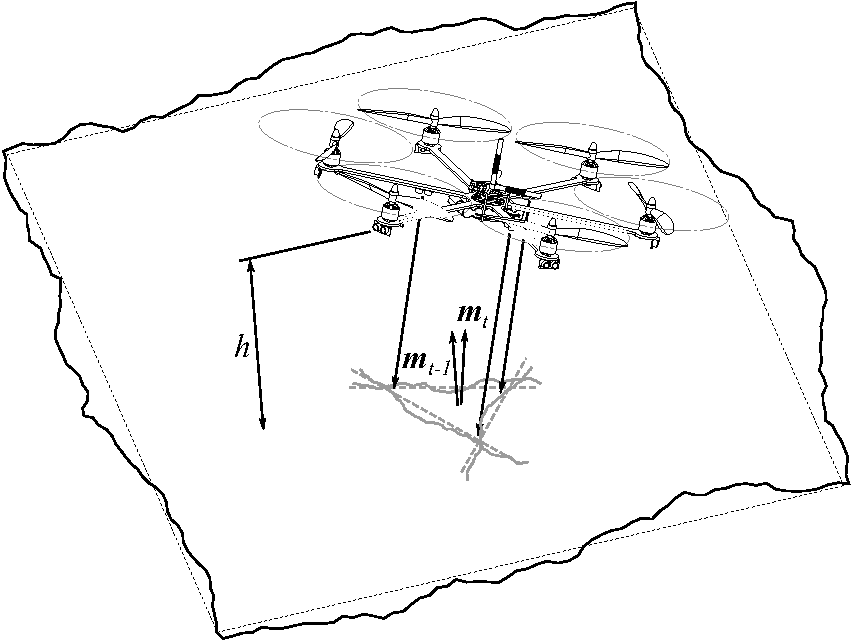
\includegraphics[scale=0.65]{ch3/img/altitude_keep.pdf}
	\caption{Altitude keeping problem}
	\forceversofloat
\end{figure}
\FloatBarrier
We can model the problem taking into account attitude dynamic and vertical dynamic of the VTOL, from which we know also the rotation matrix of the drone. The plane of the avalanche could be approximated through the orthogonal versor $\vers{m}$, projected in the drone reference frame. The problem, inserting $\vers{m}$ into the state vector, becomes equivalent to a \emph{SLAM}\sidenote[][-1cm]{\emph{SLAM}: Simultaneous Localization And Mapping} problem.

The state is:
\renewcommand{\arraystretch}{1}
\begin{equation}
\hexastate = \vettore{\hexastate \\ \vers{m}_b}
\end{equation}
\renewcommand{\arraystretch}{1.75}
and the covariance matrix of the state derives from covariance of the position system at which must be added a covarianc ematrix on the knowledge of ${\vers{m}_b = \rotmat^{T} \vers{m}}$. We could use three range finder directed to the ground, under the drone, that allow us to define three points on the surface. A model for the measurement function uses some simple algebraic definitions: given three points that belong to the plane, $\{A,\, B,\, C\}$, the normal is:
\begin{equation}
\vers{m} = \dfrac{(A-B)\times(B-C)}{\abs{(A-B)\times(B-C)}}
\end{equation}

Once normal is know, it could be used to implement a tracking control that maintains a certain distance on the normal vector. As already said, the performance of this algorithm depends directly from the estimation of the covariance matrix for measurement, and upon the sonar response due to variation of snow on the field.
%\FloatBarrier7